Der Großteil, neben der Feldarbeit, dreht sich bei der Landwirtschaft um den
Viehbetrieb. Hier gibt es bereits einige Automatisierungen, wie zum Beispiel
Melkstraßen, wo Kühe mithilfe von Melkrobotern nacheinander vollautomatisch
gemolken werden. Was zudem leicht zu automatisieren ist, ist die Ernährung
jeglicher Tierarten.\\ Man benötigt lediglich ein System, das Futter von großen
Lagerbehältern zu den Ställen/Gehegen bringt. Das kann je nach Bauernhof
unterschiedlich aussehen. Die einfachste Umsetzung wäre hierbei meiner Hinsicht
nach ein höher gelegenes Schienensystem. Damit gibt es keine Behinderung der
sonstigen Arbeit, und das komplette System kann mittels eines
Mikrokontrollers , wie zum Beispiel eines Raspberrys, gesteuert werden. Die
herkömmlichsten Roboter gleichen jedoch herkömmlichen Futtermischwägen, welche
vollautomatisiert durch die Ställe fahren. (Abbildung \ref{fig:futterroboter})

\begin{figure}[ht]
    \centering
    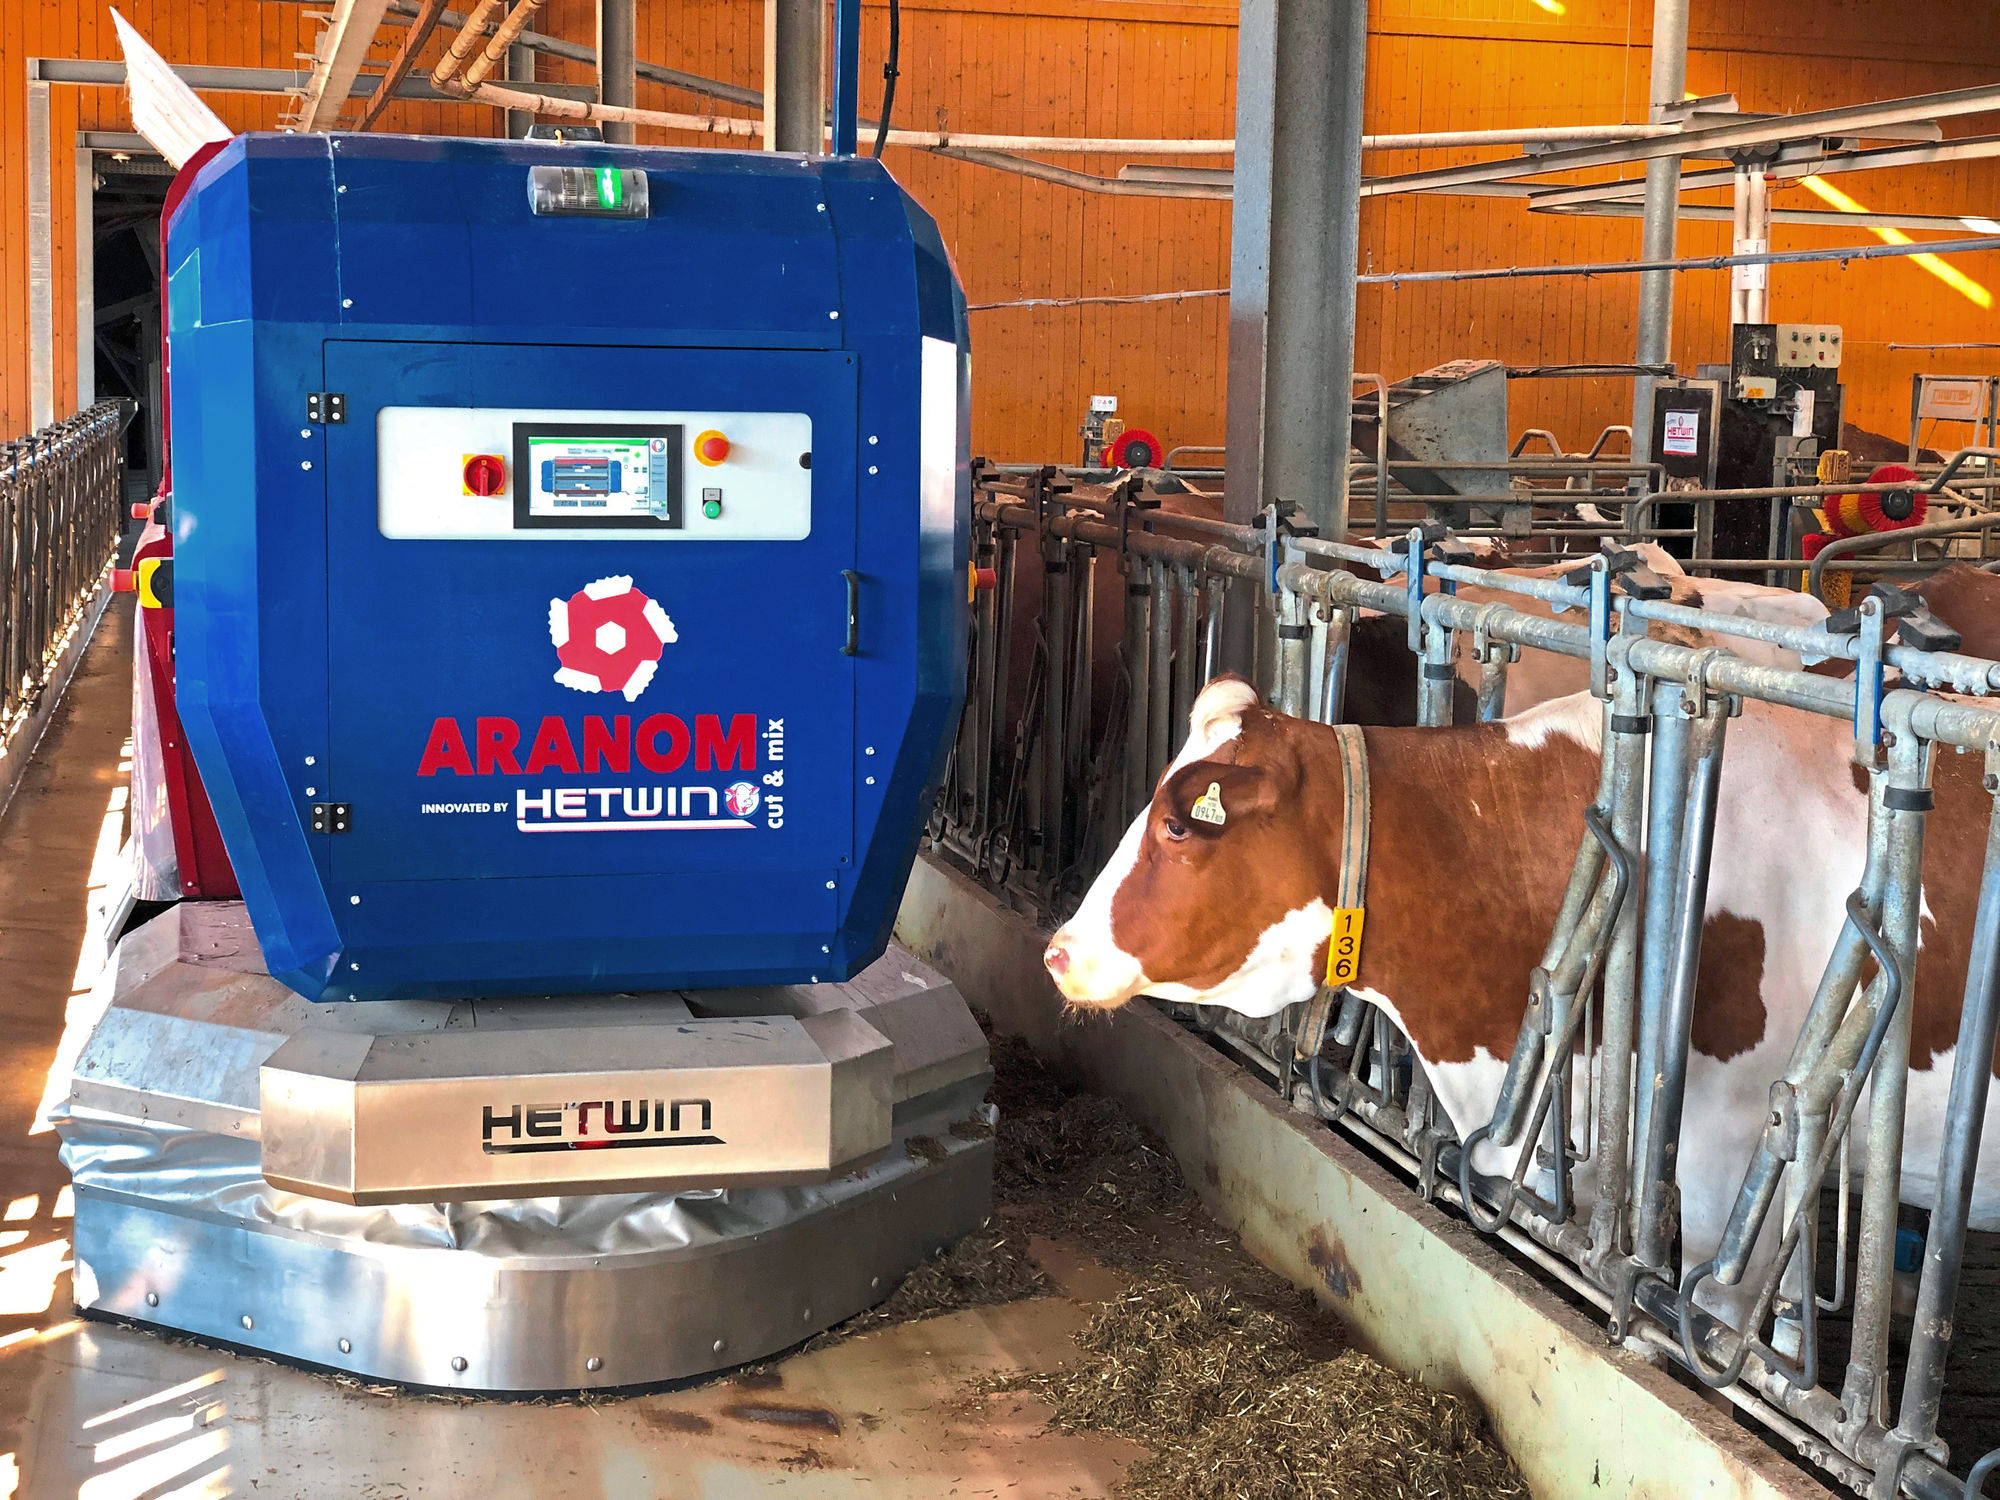
\includegraphics[width=0.7\textwidth]{bilder/futterroboter.jpg}
    \caption[Futterroboter in Kuhstall]{Futterroboter in Kuhstall \cite{Futterroboter}}
    \label{fig:futterroboter}
\end{figure}

Ein weiteres großes Anwendungsgebiet bei der Tierpflege sind
Stallreinigungsroboter (Abbildung \ref{fig:rroboter}).

\begin{figure}[ht]
    \centering
    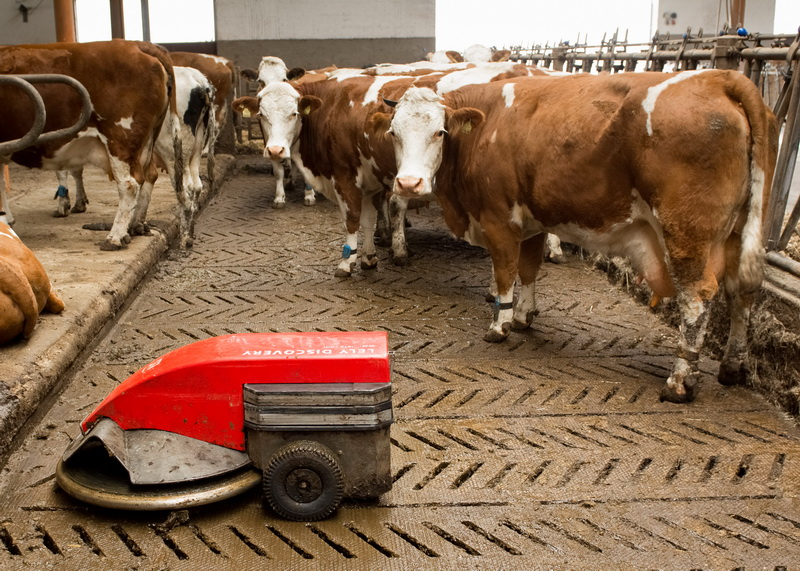
\includegraphics[width=0.7\textwidth]{bilder/Spaltenroboter_agrarfoto.com_.jpg}
    \caption[Reinigungsroboter in Kuhstall]{Reinigungsroboter in Kuhstall \cite{Reinigungsroboter}}
    \label{fig:rroboter}
\end{figure}

Die Roboter sind speziell für den Einsatz in Kuhställen
entwickelt worden. Sie sind mit Sensoren ausgestattet, um Hindernisse zu
erkennen und sicher zu navigieren. Die Reinigungsfunktionen umfassen das
Entfernen von Kot und Urin, das Kehren des Bodens und sogar das Spülen der
Laufflächen. Durch die regelmäßige Reinigung werden Keime und Krankheitserreger
reduziert, was zu einer gesünderen Umgebung für die Kühe führt. Ein weiterer
großer Vorteil von Reinigungsrobotern im Kuhstall ist der Komfort für die Kühe.
Saubere Laufflächen sorgen dafür, dass die Kühe sich wohler fühlen und weniger
anfällig für Verletzungen oder Krankheiten sind. Durch die regelmäßige
Entfernung von Kot und Urin wird zudem die Entstehung von Ammoniakgeruch
reduziert, was die Atemwege der Kühe schont.Durch die automatisierte Reinigung
können Landwirte ihre Zeit effizienter nutzen und sich auf andere wichtige
Aufgaben konzentrieren. Zudem kann die Produktivität gesteigert werden, da die
Kühe in einer sauberen Umgebung gesünder sind und bessere Milch- und
Fleischleistungen erbringen können.\cite{agrarheute}